\documentclass{beamer}
\usefonttheme[onlymath]{serif}
\usepackage[T1]{fontenc}
\usepackage[utf8]{inputenc}
\usepackage[english, icelandic]{babel}
\usepackage{amsmath}
\usepackage{amssymb}
\usepackage{amsthm}
\usepackage{gensymb}
\usepackage{parskip}
\usepackage{mathtools}
\usepackage{listings}
\usepackage{hyperref}
\usepackage{graphicx}
\usepackage{color}
\usepackage{enumerate}
\usepackage{tikz}
\usetikzlibrary{calc}
\usetikzlibrary{positioning}
\usetikzlibrary{angles}
\usetikzlibrary{shapes}
\usetikzlibrary{arrows}
\usepackage{verbatim}
\usepackage{multicol}
\usepackage{array}
\usepackage{minted}
\parskip 0pt

\usepackage{colortbl}
\usepackage{pgf}
\usepackage{pgfkeys}
\usetikzlibrary{fpu}
\usepackage{tkz-euclide}

\DeclareMathOperator{\lcm}{lcm}
\newcommand\floor[1]{\left\lfloor#1\right\rfloor}
\newcommand\ceil[1]{\left\lceil#1\right\rceil}
\newcommand\abs[1]{\left|#1\right|}
\newcommand\p[1]{\left(#1\right)}
\newcommand\sqp[1]{\left[#1\right]}
\newcommand\cp[1]{\left\{#1\right\}}
\newcommand\norm[1]{\left\lVert#1\right\rVert}
\renewcommand\Im{\operatorname{Im}}
\renewcommand\Re{\operatorname{Re}}

\usetheme{metropolis}
\definecolor{dark yellow}{rgb} {0.6,0.6,0.0}
\definecolor{dark green}{rgb} {0.0,0.6,0.0}

\graphicspath{{myndir/}}

\tikzstyle{vertex}=[circle,fill=black!50,minimum size=15pt,inner sep=0pt, font=\small]
\tikzstyle{selected vertex} = [vertex, fill=red!24]
\tikzstyle{edge} = [draw,thick,-]
\tikzstyle{dedge} = [draw,thick,->]
\tikzstyle{weight} = [font=\scriptsize,pos=0.5]
\tikzstyle{selected edge} = [draw,line width=2pt,-,red!50]
\tikzstyle{ignored edge} = [draw,line width=5pt,-,black!20]

\tikzset{
  treenode/.style = {align=center, inner sep=0pt, text centered,
    font=\sffamily},
  vertex/.style = {treenode, circle, black, font=\sffamily\bfseries\tiny, draw=black, text width=1.8em},% arbre rouge noir, noeud noir
  rvertex/.style = {treenode, circle, black, font=\sffamily\bfseries\tiny, draw=red, text width=1.8em},% arbre rouge noir, noeud noir
}

\definecolor{offwhite}{RGB}{249,242,215}
\definecolor{foreground}{HTML}{23373b}
\definecolor{background}{RGB}{24,24,24}
\definecolor{title}{RGB}{107,174,214}
\definecolor{gray}{RGB}{155,155,155}
\definecolor{subtitle}{RGB}{102,255,204}
\definecolor{lolight}{RGB}{155,155,155}
\definecolor{green}{RGB}{125,250,125}

\definecolor{hilight}{RGB}{235,129,27}
\definecolor{vhilight}{HTML}{14B03D}

\def\hepta{\draw[foreground](A) -- (B) -- (C) -- (D) -- (E) -- (F) -- (G) -- cycle;}

\newcommand{\slice}[1]{%
    \hepta
    \draw[foreground] \foreach \x/\y in {#1} {(\x)--(\y)};
}

\title{Geometry}
\author{Atli FF}
\institute{\href{http://ru.is/td}{School of Computer Science} \\[2pt] \href{http://ru.is}{Reykjavík University}}
\titlegraphic{\hfill
\includegraphics[height=0.6cm]{../../shared/kattis}}

\begin{document}
\maketitle

\begin{frame}[plain]{Today's material}
    \vspace{40pt}
    \begin{itemize}
      \item Trigonometry
      \item Geometry
      \item Computational geometry
    \end{itemize}
\end{frame}

\begin{frame}[plain]{Trigonometry}
    \begin{columns}
        \begin{column}{0.7\textwidth}
            \begin{itemize}
                \item Before we even dive into the geometry and how to do it on a computer, let's jog your memories.
                \item You should all hopefully be familiar with the trigonometric functions.
                \item We consider a triangle to be right-angled if it has a corner that's $90^{\circ}$.
                \item For such triangles we have:
                \begin{itemize}
                    \item $\dfrac{A}{L} = \cos\theta$.
                    \item $\dfrac{M}{L} = \sin\theta$.
                    \item $\dfrac{M}{A} = \dfrac{M}{L}\dfrac{L}{A} = \dfrac{\sin\theta}{\cos\theta} = \tan\theta$.
                \end{itemize}
                \item We also have the pythagorean theorem $L^2 = A^2 + M^2$.
            \end{itemize}
        \end{column}
		\begin{column}{0.3\textwidth}
			\scalebox{0.75} {
				\begin{tikzpicture}
					\coordinate (A) at (0, 0) {};
					\coordinate (B) at (4, 0) {};
					\coordinate (C) at (0, 3) {};
					\node at (3.2, 0.3) {$\theta$};

					\draw (A) -- node[below] {$A$} (B);
					\draw (B) -- node[above] {$L$} (C);
					\draw (C) -- node[left] {$M$} (A);
					\draw pic[draw, angle radius = 0.5cm] {angle=C--B--A};
                \end{tikzpicture}
            }
        \end{column}
    \end{columns}
\end{frame}

\begin{frame}[plain]{More trig}
	\begin{columns}
		\begin{column}{0.7\textwidth}
			\begin{itemize}
				\item More generally we have:
				\begin{itemize}
					\item $\dfrac{\sin a}{A} = \dfrac{\sin b}{B} = \dfrac{\sin c}{C}$ (sine law).
					\item $A^2 = B^2 + C^2 - 2BC\cos a$ (cosine law)
                \end{itemize}
				\item {\bf Exercise:} Prove the pythagorean theorem using the cosine law.
            \end{itemize}
        \end{column}
		\begin{column}{0.3\textwidth}
			\scalebox{0.8} {
				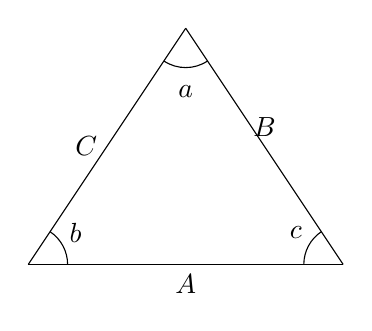
\begin{tikzpicture}
					\coordinate (A) at (0, 0) {};
					\node at (0.60, 0.4) {$b$};
					\coordinate (B) at (4, 0) {};
					\node at (3.4, 0.4) {$c$};
					\coordinate (C) at (2, 3) {};
					\node at (2, 2.2) {$a$};

					\draw (A) -- node[below] {$A$} (B);
					\draw (B) -- node[above] {$B$} (C);
					\draw (C) -- node[left] {$C$} (A);
					\draw pic[draw, angle radius = 0.5cm] {angle=B--A--C};
					\draw pic[draw, angle radius = 0.5cm] {angle=A--C--B};
					\draw pic[draw, angle radius = 0.5cm] {angle=C--B--A};
                \end{tikzpicture}
			}
        \end{column}
    \end{columns}
\end{frame}

\begin{frame}[plain]{Example: NN and the Optical Illusion}
	\begin{itemize}
        \item You are given an integer $n$ and a real number $r$.
        \item You then draw a circle of radius $r$.
        \item You then want to draw $n$ circles of the same size tangent to the outside of this circle and such that they are tangent to their neighbours.
        \item What radius will the outer circles have?
    \end{itemize}
\end{frame}

\begin{frame}[plain]{$N = 6$ image}
	\center
	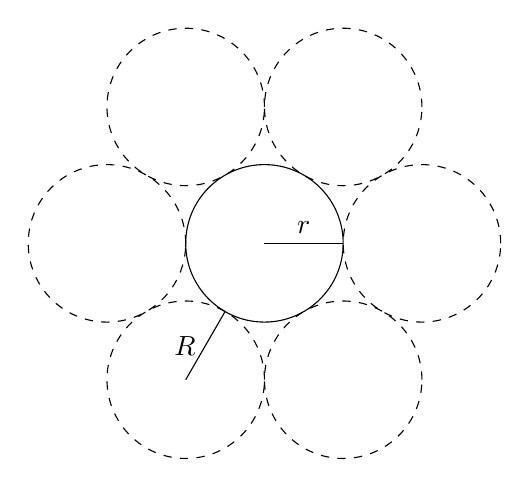
\begin{tikzpicture}
		\coordinate (O) at (0, 0) {};
		\coordinate (A) at (1, 0) {};
		\coordinate (B) at (-1, 0) {};
		\coordinate (C) at (0.5, 0.8660254038) {};
		\coordinate (D) at (0.5, -0.8660254038) {};
		\coordinate (E) at (-0.5, -0.8660254038) {};
		\coordinate (F) at (-0.5, 0.8660254038) {};

		\coordinate (AA) at (2,0) {};
		\coordinate (BB) at (-2,0) {};
		\coordinate (CC) at (1,1.732050808) {};
		\coordinate (DD) at (1,-1.732050808) {};
		\coordinate (EE) at (-1,-1.732050808) {};
		\coordinate (FF) at (-1,1.732050808) {};

		\draw (O) circle (1);
		\draw[dashed] (AA) circle (1);
		\draw[dashed] (BB) circle (1);
		\draw[dashed] (CC) circle (1);
		\draw[dashed] (DD) circle (1);
		\draw[dashed] (EE) circle (1);
		\draw[dashed] (FF) circle (1);

		\draw (O) -- node[above] {$r$} (A);
		\draw (E) -- node[left] {$R$} (EE);
    \end{tikzpicture}
\end{frame}

\begin{frame}[plain]{Towards a solution}
    We see that the distance from the center of the circle in the middle to the
    center of an outer circle is $r + R$. We thus get an isosceles triangle.
	\center
	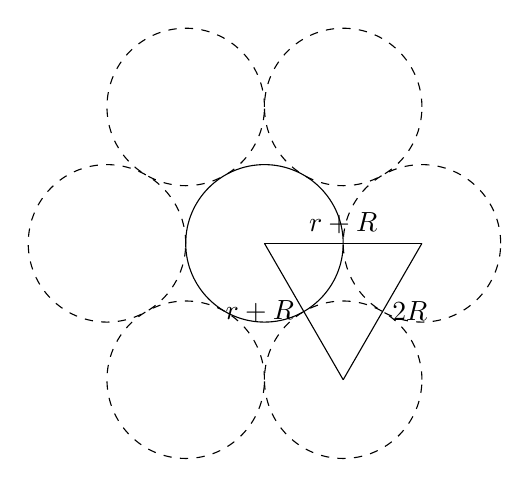
\begin{tikzpicture}
		\coordinate (O) at (0, 0) {};
		\coordinate (A) at (1, 0) {};
		\coordinate (B) at (-1, 0) {};
		\coordinate (C) at (0.5, 0.8660254038) {};
		\coordinate (D) at (0.5, -0.8660254038) {};
		\coordinate (E) at (-0.5, -0.8660254038) {};
		\coordinate (F) at (-0.5, 0.8660254038) {};

		\coordinate (AA) at (2,0) {};
		\coordinate (BB) at (-2,0) {};
		\coordinate (CC) at (1,1.732050808) {};
		\coordinate (DD) at (1,-1.732050808) {};
		\coordinate (EE) at (-1,-1.732050808) {};
		\coordinate (FF) at (-1,1.732050808) {};

		\draw (O) circle (1);
		\draw[dashed] (AA) circle (1);
		\draw[dashed] (BB) circle (1);
		\draw[dashed] (CC) circle (1);
		\draw[dashed] (DD) circle (1);
		\draw[dashed] (EE) circle (1);
		\draw[dashed] (FF) circle (1);

		\draw (O) -- node[above] {$r + R$} (AA);
		\draw (O) -- node[left] {$r + R$} (DD);
		\draw (AA) -- node[right] {$2R$} (DD);
    \end{tikzpicture}
\end{frame}

\begin{frame}[plain]{Closer and closer}
	\begin{itemize}
	    \item Now we have
		$\theta = \dfrac{360^{\circ}}{n}$
		and
		$\omega = \dfrac{180^{\circ} - \theta}{2}$.
    \end{itemize}
	\center
	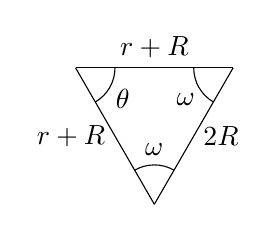
\begin{tikzpicture}
		\coordinate (O) at (0, 0) {};
		\coordinate (A) at (1, 0) {};
		\coordinate (B) at (-1, 0) {};
		\coordinate (C) at (0.5, 0.8660254038) {};
		\coordinate (D) at (0.5, -0.8660254038) {};
		\coordinate (E) at (-0.5, -0.8660254038) {};
		\coordinate (F) at (-0.5, 0.8660254038) {};

		\coordinate (AA) at (2,0) {};
		\coordinate (BB) at (-2,0) {};
		\coordinate (CC) at (1,1.732050808) {};
		\coordinate (DD) at (1,-1.732050808) {};
		\coordinate (EE) at (-1,-1.732050808) {};
		\coordinate (FF) at (-1,1.732050808) {};

		\draw (O) -- node[above] {$r + R$} (AA);
		\draw (O) -- node[left] {$r + R$} (DD);
		\draw (AA) -- node[right] {$2R$} (DD);

		\draw pic[draw, angle radius = 0.5cm] {angle=O--AA--DD};
		\draw pic[draw, angle radius = 0.5cm] {angle=AA--DD--O};
		\draw pic[draw, angle radius = 0.5cm] {angle=DD--O--AA};
		\node at (0.6, -0.4) {$\theta$};
		\node at (1, -1.032050808) {$\omega$};
		\node at (1.4, -0.4) {$\omega$};
    \end{tikzpicture}
\end{frame}

\begin{frame}[plain]{Solution}
	\begin{itemize}
		\item Finally the law of sines gives us
		\begin{align*}
			\frac{2R}{\sin \theta} = \frac{r + R}{\sin \omega}
				& \Rightarrow 2R\sin\omega = r\sin\theta + R\sin\theta\\
				& \Rightarrow 2R\sin\omega - R\sin\theta = r\sin\theta \\
				& \Rightarrow R = \frac{r\sin\theta}{2\sin\omega - \sin\theta}.
        \end{align*}
    \end{itemize}
	\center
	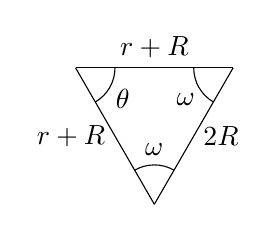
\begin{tikzpicture}
		\coordinate (O) at (0, 0) {};
		\coordinate (A) at (1, 0) {};
		\coordinate (B) at (-1, 0) {};
		\coordinate (C) at (0.5, 0.8660254038) {};
		\coordinate (D) at (0.5, -0.8660254038) {};
		\coordinate (E) at (-0.5, -0.8660254038) {};
		\coordinate (F) at (-0.5, 0.8660254038) {};

		\coordinate (AA) at (2,0) {};
		\coordinate (BB) at (-2,0) {};
		\coordinate (CC) at (1,1.732050808) {};
		\coordinate (DD) at (1,-1.732050808) {};
		\coordinate (EE) at (-1,-1.732050808) {};
		\coordinate (FF) at (-1,1.732050808) {};

		\draw (O) -- node[above] {$r + R$} (AA);
		\draw (O) -- node[left] {$r + R$} (DD);
		\draw (AA) -- node[right] {$2R$} (DD);

		\draw pic[draw, angle radius = 0.5cm] {angle=O--AA--DD};
		\draw pic[draw, angle radius = 0.5cm] {angle=AA--DD--O};
		\draw pic[draw, angle radius = 0.5cm] {angle=DD--O--AA};
		\node at (0.6, -0.4) {$\theta$};
		\node at (1, -1.032050808) {$\omega$};
		\node at (1.4, -0.4) {$\omega$};
    \end{tikzpicture}
\end{frame}

\begin{frame}[plain]
  \begin{columns}
    \begin{column}{0.5\textwidth}
      \begin{figure}
        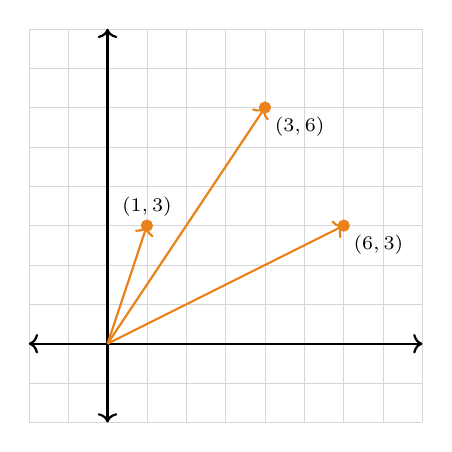
\begin{tikzpicture}
          \draw[step=.5cm, very thin, foreground, opacity=0.2] (0,0) grid (5,5);
          \draw[thick, ->] (1,1) -- (0,1);
          \draw[thick, ->] (1,1) -- (5,1);
          \draw[thick, ->] (1,1) -- (1,0);
          \draw[thick, ->] (1,1) -- (1,5);

          \visible<2->{
            \draw[hilight,fill] (3,4) circle[radius=2pt];
            \draw (3,4) node[anchor=north west] {\scriptsize$(3,6)$};
            \draw[hilight,fill] (4,2.5) circle[radius=2pt];
            \draw (4,2.5) node[anchor=north west] {\scriptsize$(6,3)$};
            \draw[hilight,fill] (1.5,2.5) circle[radius=2pt];
            \draw (1.5,2.5) node[anchor=south] {\scriptsize$(1,3)$};
          }

          \visible<3->{
            \draw[hilight,thick,->] (1,1) -- (3,4);
            \draw[hilight,thick,->] (1,1) -- (4,2.5);
            \draw[hilight,thick,->] (1,1) -- (1.5,2.5);
          }
        \end{tikzpicture}
      \end{figure}
    \end{column}
    \begin{column}{0.5\textwidth}
      \begin{itemize}
        \onslide<2->
        \item Points are represented by a pair of numbers, $(x,y)$.
        \onslide<3->
        \item Vectors are represented in the same way.
        \item Thinking of points as vectors allows us to do many things.
      \end{itemize}
    \end{column}
  \end{columns}
\end{frame}

\begin{frame}[plain,fragile]
  %Points and vectors can be represented by a pair of numbers, $x$ and $y$.
  \begin{columns}
    \begin{column}{0.5\textwidth}
      \begin{figure}
        \footnotesize
        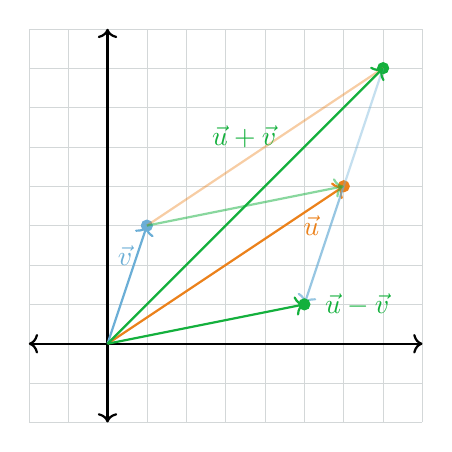
\begin{tikzpicture}
          \draw[step=.5cm, very thin, foreground, opacity=0.2] (0,0) grid (5,5);
          \draw[thick, ->] (1,1) -- (0,1);
          \draw[thick, ->] (1,1) -- (5,1);
          \draw[thick, ->] (1,1) -- (1,0);
          \draw[thick, ->] (1,1) -- (1,5);

          \draw[hilight,fill] (4,3) circle[radius=2pt];
          \draw[title,fill] (1.5,2.5) circle[radius=2pt];

          \draw[hilight,thick,->] (1,1) -- node[right=3pt, near end] {$\vec u$} (4,3);
          \draw[title,thick,->] (1,1) -- node[left=-2pt,near end] {$\vec v$} (1.5,2.5);

          \visible<3>{
            \draw[vhilight,fill] (4.5,4.5) circle[radius=2pt];
            \draw[hilight,thick,opacity=0.4] (1.5,2.5) -- (4.5, 4.5);
            \draw[title,thick,opacity=0.4] (4,3) -- (4.5, 4.5);
            \draw[vhilight,thick,->] (1,1) -- node[left=10pt, near end] {$\vec u + \vec v$} (4.5, 4.5);
          }
          \visible<5>{
            \draw[title,thick,->, opacity=0.7] (4,3) -- (3.5,1.5);
            \draw[vhilight,fill] (3.5,1.5) circle[radius=2pt];
            \draw (3.5,1.5) node[right=4pt] {{\color{vhilight}$\vec u - \vec v$}};
            \draw[vhilight,thick,->] (1,1) --  (3.5, 1.5);
            \draw[vhilight,thick,->, opacity=0.5] (1.5,2.5) -- (4,3);
          }
        \end{tikzpicture}
      \end{figure}
    \end{column}
    \begin{column}{0.5\textwidth}
      %\footnotesize
      \begin{itemize}
        \onslide<2->
        \item Simplest operation, addition is defined as
          \[
            {\color{title!80!black}
            \begin{pmatrix}
              x_0 \\
              y_0
            \end{pmatrix}
            }
            +
            {\color{hilight!90!black}
            \begin{pmatrix}
              x_1 \\
              y_1
            \end{pmatrix}
            }
            =
            {\color{vhilight!80!black}
            \begin{pmatrix}
              x_0 + x_1 \\
              y_0 + y_1
            \end{pmatrix}
            }
          \]
        \onslide<4->
        \item Subtraction is defined in the same manner
          \[
            {\color{hilight!90!black}
            \begin{pmatrix}
              x_0 \\
              y_0
            \end{pmatrix}
            }
            -
            {\color{title!80!black}
            \begin{pmatrix}
              x_1 \\
              y_1
            \end{pmatrix}
            }
            =
            {\color{vhilight!80!black}
            \begin{pmatrix}
              x_0 - x_1 \\
              y_0 - y_1
            \end{pmatrix}
            }
          \]
      \end{itemize}
    \end{column}
  \end{columns}
\end{frame}

\begin{frame}[plain,fragile]
  \begin{minted}{cpp}
struct point {
    double x, y;
    point(double _x, double _y) { 
        x = _x, y = _y;
    }

    point operator+(const point &oth){
        return point(x + oth.x, y + oth.y);
    }

    point operator-(const point &oth){
        return point(x - oth.x, y - oth.y);
    }
};
  \end{minted}
\end{frame}

\begin{frame}[plain,fragile]
  \vspace{20pt}
  \ldots or we could use the \texttt{complex<double>} class. 
  \begin{minted}{cpp}
using points = complex<double>;
  \end{minted}
  \onslide<2->
  \vspace{10pt}
  The \texttt{complex} class in \texttt{C++} and \texttt{Java} has methods defined for
  \begin{itemize}
    \item Addition
    \item Subtraction
    \item Multiplication by a scalar
    \item Length
    \item Trigonometric functions
    \item And much more!
  \end{itemize}
\end{frame}

\begin{frame}[plain]{Complex numbers}
	\begin{itemize}
        \item We define $\mathbb{C} \coloneqq \mathbb{R} \times \mathbb{R}$.
        \item Then we define addition on $\mathbb{C}$ such that for $(a, b), (c, d) \in \mathbb{C}$ we get
			\[
				(a, b) + (c, d) = (a + c, b + d).
			\]
        \item We also define multiplication on $\mathbb{C}$ such that for $(a, b), (c, d) \in \mathbb{C}$ we get
			\[
				(a, b) \cdot (c, d) = (ac - bd, ad + bc).
			\]
        \item We usually denote $(0, 1) \in \mathbb{C}$ by $i$ and $(x, y) \in \mathbb{C}$ by $x + yi$.
        \item Note that $(x, y) = (x, 0) + i \cdot (y, 0)$ here.
        \item We call these numbers in $\mathbb{C}$ \emph{complex numbers}.
    \end{itemize}
\end{frame}

\begin{frame}[plain]{Complex numbers ctd.}
	\begin{itemize}
        \item If $z = x + yi \in \mathbb{C}$ then
		\begin{itemize}
            \item We call $x$ the \emph{real part} of $z$ and $y$ the \emph{imaginary part} of $z$.
            \item We define the \emph{magnitude} of $z$ by $|z| = \sqrt{x^2 + y^2}$.
            \item We call $x - yi$ the \emph{conjugate} of $z$, denoted by $\overline{z}$.
            \item We call the angle $(x, y)$ makes with the positive $x$-axis the \emph{argument} of $z$ and
                denote it by $\operatorname{Arg}(z)$.
        \end{itemize}
    \end{itemize}
\end{frame}

\begin{frame}[plain]{Operations}
	\begin{itemize}
        \item Let $w, z \in \mathbb{C}$.
        \item Then $w + z$ will be $z$ translated by $w$, as if we were adding vectors.
        \item If $|w| = 1$ then $z \cdot w$ will be $z$ rotated around $0$ by $\operatorname{Arg}(w)$ radians.
        \item If $|z| = r$ and $\operatorname{Arg}(z) = \theta$ we can write $z = re^{i\theta}$.
        \item If $z = r_1e^{i\theta_1}$ and $w = r_2e^{i\theta_2}$ then $z \cdot w = r_1 r_2 e^{i(\theta_1 + \theta_2)}$.
    \end{itemize}
\end{frame}

\begin{frame}[plain]{Using complex in C++}
    \begin{itemize}
        \item Usually we do \texttt{using point = complex<double>}
        \item Then we can initialize a point with \texttt{point z(x, y)}
        \begin{itemize}
            \item \texttt{real(z)} returns the $x$-coordinate
            \item \texttt{imag(z)} returns the $y$-coordinate
            \item \texttt{abs(z)} returns the magnitude $|z|$
            \item \texttt{abs(z - w)} returns the distance from $z$ to $w$
            \item \texttt{arg(z)} returns the argument of $z$
            \item \texttt{conj(z)} returns the conjugate $\overline{z}$
        \end{itemize}
    \end{itemize}
\end{frame}

\begin{frame}[plain]{Example}
	\begin{itemize}
        \item Let us consider a problem.
        \item You start at $(0, 0)$ and get a sequence of commands.
        \item All the commands consist of a single letter and a number. The commands are:
		\begin{itemize}
			\item ...\texttt{f x} you move forward $x$ meters..
			\item ...\texttt{b x} you move backwards $x$ meters.
			\item ...\texttt{r x} you rotate $x$ radians to the right.
			\item ...\texttt{l x} you rotate $x$ radians to the left.
        \end{itemize}
        \item How far from $(0, 0)$ do you end up after following the commands?
    \end{itemize}
\end{frame}

\begin{frame}[plain]{Solution}
	\begin{itemize}
        \item If we are stood at $p \in \mathbb{C}$ and want to take a step of $r$ meters in the direction $\theta$ we simply add $re^{i\theta}$ to $p$.
        \item What direction we are facing at the start makes no difference since it gives the same distance at the end.
    \end{itemize}
\end{frame}

\begin{frame}[plain, fragile]{Code}
\small
    \begin{minted}{cpp}
#include<bits/stdc++.h>
using namespace std;
using point = complex<double>;
int main() {
    int n; cin >> n;
    double x, r = 0.0;
    point p(0, 0);
    while (n--) {
        char c; cin >> c >> x;
        if (c == 'f')      p += x*exp(1i*r);
        else if (c == 'b') p -= x*exp(1i*r);
        else if (c == 'l') r += x;
        else if (c == 'r') r -= x;
        else assert(0);
	}
    cout << setprecision(15) << abs(p) << endl;
}
    \end{minted}
\end{frame}

\begin{frame}[plain,fragile]
  \begin{columns}
    \begin{column}{0.5\textwidth}
      \begin{figure}
        \footnotesize
        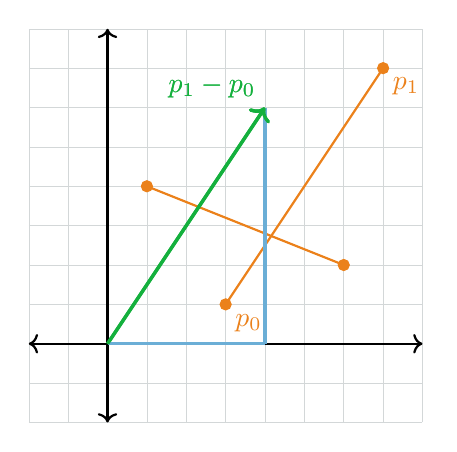
\begin{tikzpicture}
          \draw[step=.5cm, very thin, foreground, opacity=0.2] (0,0) grid (5,5);
          \draw[thick, ->] (1,1) -- (0,1);
          \draw[thick, ->] (1,1) -- (5,1);
          \draw[thick, ->] (1,1) -- (1,0);
          \draw[thick, ->] (1,1) -- (1,5);
          \visible<1>{
            \draw[hilight,fill] (1.5,3) circle[radius=2pt];
            %\draw (1.5,3) node[anchor=south] {\scriptsize$(1,4)$};
            \draw[hilight,fill] (4,2) circle[radius=2pt];
            %\draw (4,2) node[anchor=north west] {\scriptsize$(6,2)$};
            \draw[hilight,thick] (1.5,3) -- (4,2);
          }

          \visible<1-2>{
            \draw[hilight,fill] (2.5,1.5) circle[radius=2pt];
            \draw[hilight,fill] (4.5,4.5) circle[radius=2pt];
            \draw[hilight,thick] (2.5,1.5) -- (4.5,4.5);
          }

          \visible<2>{
            \draw (2.5,1.5) node[anchor=north west] {{\color{hilight}$p_0$}};
            \draw (4.5,4.5) node[anchor=north west] {{\color{hilight}$p_1$}};
            \draw[vhilight,very thick,->] (1,1) -- (3,4);
            \draw (3,4) node[anchor=south east] {{\color{vhilight}$p_1 - p_0$}};
          }

          \visible<3>{
            \draw[title,very thick] (1,1) -- (3,1);
            \draw[title,very thick] (3,1) -- (3,4);
            \draw[vhilight,very thick,->] (1,1) -- (3,4);
            \draw (3,4) node[anchor=south east] {{\color{vhilight}$p_1 - p_0$}};
          }
        \end{tikzpicture}
      \end{figure}
    \end{column}
    \begin{column}{0.55\textwidth}
      \begin{itemize}
        \item Line segments are represented by a pair of points, $((x_0,y_0), (x_1,y_1))$.
      \end{itemize}
    \end{column}
  \end{columns}
\end{frame}

\begin{frame}[plain,fragile]
  \begin{columns}
    \begin{column}{0.5\textwidth}
      \begin{figure}
        \footnotesize
        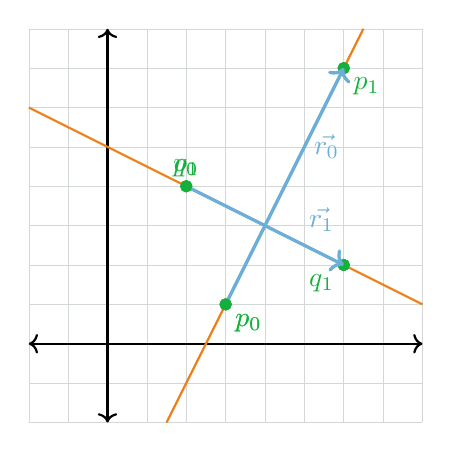
\begin{tikzpicture}
          \draw[step=.5cm, very thin, foreground, opacity=0.2] (0,0) grid (5,5);
          \draw[thick, ->] (1,1) -- (0,1);
          \draw[thick, ->] (1,1) -- (5,1);
          \draw[thick, ->] (1,1) -- (1,0);
          \draw[thick, ->] (1,1) -- (1,5);

          \draw[hilight,fill] (2,3) circle[radius=2pt];
          \draw[hilight,fill] (4,2) circle[radius=2pt];
          \draw[hilight,thick] (2,3) -- (4,2);

          \draw[hilight,fill] (2.5,1.5) circle[radius=2pt];
          \draw[hilight,fill] (4,4.5) circle[radius=2pt];
          \draw[hilight,thick] (2.5,1.5) -- (4,4.5);

          \visible<2>{
            \draw (4,2) node[anchor=north east] {{\color{vhilight}$q_1$}};
            \draw (4,4.5) node[anchor=north west] {{\color{vhilight}$p_1$}};
            \draw (2,3) node[anchor=south] {{\color{vhilight}$q_0$}};
            \draw (2.5,1.5) node[anchor=north west] {{\color{vhilight}$p_0$}};
          }
          \visible<2->{
            \draw[hilight,thick] (5,1.5) -- (0,4);
            \draw[hilight,thick] (1.75,0) -- (4.25,5);

            \draw[vhilight,fill] (2,3) circle[radius=2pt];
            \draw[vhilight,fill] (4,2) circle[radius=2pt];

            \draw[vhilight,fill] (2.5,1.5) circle[radius=2pt];
            \draw[vhilight,fill] (4,4.5) circle[radius=2pt];
          }

          \visible<3->{
            \draw[vhilight,fill] (4,2) circle[radius=2pt];
            \draw[title,very thick,->] (2,3) -- (4,2);
            \draw[vhilight,fill] (2,3) circle[radius=2pt];

            \draw[vhilight,fill] (4,4.5) circle[radius=2pt];
            \draw[title,very thick,->] (2.5,1.5) -- (4,4.5);
            \draw[vhilight,fill] (2.5,1.5) circle[radius=2pt];

            \draw (2,3) node[anchor=south] {{\color{vhilight}$p_1$}};
            \draw (2.5,1.5) node[anchor=north west] {{\color{vhilight}$p_0$}};

            \draw (3.5,3.5) node[anchor=west] {{\color{title}$\vec{r_0}$}};
            \draw (4,2.3) node[anchor=south east] {{\color{title}$\vec{r_1}$}};
          }
        \end{tikzpicture}
      \end{figure}
    \end{column}
    \begin{column}{0.6\textwidth}
      %\vspace{20pt}
      \begin{itemize}
        \item Line representation same as line segments.
        \onslide<2->
        \item Treat them as lines passing through the two points.
        \onslide<3->
        \item Or as a point and a direction vector.
          \[
            {\color{vhilight}p} + {\color{hilight}t} \cdot {\color{title}\vec{r}}
          \]
        \onslide<4->
        \vspace{-10pt}
        \item Either way
          \begin{minted}{cpp}
pair<point,point>
          \end{minted}
      \end{itemize}
    \end{column}
  \end{columns}
\end{frame}

\begin{frame}[plain,fragile]
  \begin{columns}
    \begin{column}{0.5\textwidth}
      \begin{figure}
        \footnotesize
        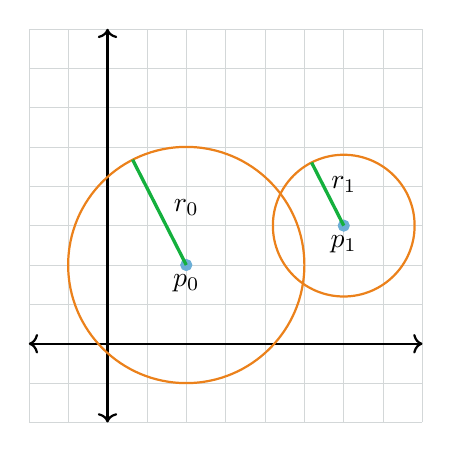
\begin{tikzpicture}
          \draw[step=.5cm, very thin, foreground, opacity=0.2] (0,0) grid (5,5);
          \draw[thick, ->] (1,1) -- (0,1);
          \draw[thick, ->] (1,1) -- (5,1);
          \draw[thick, ->] (1,1) -- (1,0);
          \draw[thick, ->] (1,1) -- (1,5);

          \draw[hilight,thick] (2,2) circle[radius=1.5cm];
          \draw[hilight,thick] (4,2.5) circle[radius=0.9cm];
          %\draw (3,4) node[anchor=north west] {\scriptsize$(3,6)$};

          \visible<2->{
            \draw[title,fill] (2,2) circle[radius=2pt];
            \draw (2,2) node[anchor=north] {$p_0$};
            \draw[title,fill] (4,2.5) circle[radius=2pt];
            \draw (4,2.5) node[anchor=north] {$p_1$};
          }

          \visible<3->{
            %\draw (2,2) -- (0,10);
            \draw[vhilight,very thick] (2,2) --  +(117:1.5cm) ;
            \draw[vhilight,very thick] (4,2.5) --  +(117:0.9cm) ;
            \draw (2,2.5) node[anchor=south] {$r_0$};
            \draw (4,2.8) node[anchor=south] {$r_1$};
          }
        \end{tikzpicture}
      \end{figure}
    \end{column}
    \begin{column}{0.5\textwidth}
      \vspace{20pt}
      \begin{itemize}
        \item Circles are very easy to represent.
        \onslide<2->
        \item Center point ${\color{title}p = (x,y)}$.
        \onslide<3->
        \item And the radius ${\color{vhilight}r}$.
        \onslide<4->
        \begin{minted}{cpp}
pair<point,double>
        \end{minted}
      \end{itemize}
    \end{column}
  \end{columns}
\end{frame}

\begin{frame}[plain]
  \vspace{20pt}
  Given two vectors 
  \[
    \vec{u} = \begin{pmatrix} x_0 \\ y_0 \end{pmatrix} \quad\quad
    \vec{v} = \begin{pmatrix} x_1 \\ y_1 \end{pmatrix}
  \]
  the dot product of $\vec{u}$ and $\vec{v}$ is defined as 
  \[
    \begin{pmatrix} x_0 \\ y_0 \end{pmatrix} \cdot
    \begin{pmatrix} x_1 \\ y_1 \end{pmatrix} = 
    x_0 \cdot x_1 + y_0 \cdot y_1
  \]
  \onslide<2->
  Which in geometric terms is
  \[
    \vec{u} \cdot \vec{v} = 
    \lvert \vec{u} \rvert \lvert \vec{v} \rvert \cos \theta
  \]
\end{frame}

%\begin{frame}[plain]
  %\begin{columns}
    %\begin{column}{0.4\textwidth}
      %\vspace{20pt}
      %\begin{figure}
        %\begin{tikzpicture}
          %\draw[fill=title!50] (0,0) -- (40:.75cm) arc (40:0:.75cm);
          %\draw[->,thick,hilight] (0,0) -- node[near end, below] {$\vec u$} (0:4cm);
          %\draw[->,thick,vhilight] (0,0) -- node[near end, left=4pt] {$\vec v$} (40:3.2cm);
          %\draw(22:0.5cm) node {\color{background}$\theta$};

          %\visible<2->{
            %\draw[dashed] (40:3.2cm) -- (0:2.45134221cm);
            %\draw[title,thick,->] (0,0) -- node[below] {$\vec{v}_{\vec{u}}$} (0:2.45134221cm);
          %}
        %\end{tikzpicture}
      %\end{figure}
    %\end{column}
    %\begin{column}{0.6\textwidth}
      %\begin{itemize}
        %\item Allows us to calculate the angle between $\vec u$ and $\vec v$.
          %\[
            %\theta = \arccos\left(\frac{\vec{u} \cdot \vec{v}}{\lvert \vec u \rvert \lvert \vec v \rvert}\right)
          %\]
        %\onslide<2->
        %\item And the projection of $\vec v$ onto $\vec u$.
          %\[
            %\vec{v}_{\vec{u}} = \left(\frac{\vec{u}\cdot\vec{v}}{\lvert u \rvert}\right) \vec{u}
          %\]
      %\end{itemize}
    %\end{column}
  %\end{columns}
%\end{frame}

\begin{frame}[plain]
  \begin{columns}
    \begin{column}{0.4\textwidth}
      \vspace{20pt}
      \begin{figure}
        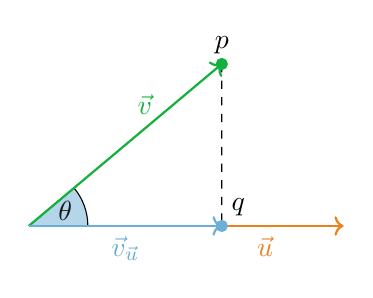
\begin{tikzpicture}
          \draw[fill=title!50] (0,0) -- (40:.75cm) arc (40:0:.75cm);
          \draw[->,thick,hilight] (0,0) -- node[near end, below] {$\vec u$} (0:4cm);
          \draw[->,thick,vhilight] (0,0) -- node[near end, left=4pt] {$\vec v$} (40:3.2cm);
          \draw(22:0.5cm) node {\color{background}$\theta$};

          \visible<2->{
            \draw[dashed] (40:3.2cm) -- (0:2.45134221cm);
            \draw[title,thick,->] (0,0) -- node[below] {$\vec{v}_{\vec{u}}$} (0:2.45134221cm);
          }

          \visible<3->{
            \draw (40:3.2cm) node[above] {$p$};
            \draw[fill,vhilight] (40:3.2cm) circle[radius=2pt];
            \draw (0:2.45134221cm) node[above right] {$q$};
            \draw[fill,title] (0:2.45134221cm) circle[radius=2pt];
          }
        \end{tikzpicture}
      \end{figure}
    \end{column}
    \begin{column}{0.6\textwidth}
      \begin{itemize}
        \only<1-2>{
          \item Allows us to calculate the angle between $\vec u$ and $\vec v$.
            \[
              \theta = \arccos\left(\frac{\vec{u} \cdot \vec{v}}{\lvert \vec u \rvert \lvert \vec v \rvert}\right)
            \]
        }
        \only<2>{
          \item And the projection of $\vec v$ onto $\vec u$.
            \[
              \vec{v}_{\vec{u}} = \left(\frac{\vec{u}\cdot\vec{v}}{\lvert u \rvert^2}\right) \vec{u}
            \]
        }
        \only<3->{
          \vspace{20pt}
          \item The closest point on $\vec{u}$ to $p$ is $q$.
        }
        \only<4->{
          \item The distance from $p$ to $\vec{u}$ is the distance from $p$ to $q$.
        }
        \only<5->{
          \item Unless $q$ is outside $\vec{u}$, then the closest point is either of the endpoints.
        }
      \end{itemize}
    \end{column}
  \end{columns}
\end{frame}

\begin{frame}[plain,fragile]
  \vspace{20pt}
  Rest of the code will use the \texttt{complex} class.
  \footnotesize
  \begin{minted}{cpp}
#define P(p) const point &p
#define L(p0, p1) P(p0), P(p1)
double dot(P(a), P(b)) { 
    return real(a) * real(b) + imag(a) * imag(b);
}
double angle(P(a), P(b), P(c)) {
    return acos(dot(b - a, c - b) / abs(b - a) / abs(c - b)); 
}
point closest_point(L(a, b), P(c), bool segment = false) {
    if (segment) {
        if (dot(b - a, c - b) > 0) return b;
        if (dot(a - b, c - a) > 0) return a;
    }
    double t = dot(c - a, b - a) / norm(b - a);
    return a + t * (b - a);
}
  \end{minted}
\end{frame}
\begin{frame}[plain]
  \vspace{20pt}
  Given two vectors
  \[
    \vec{u} = \begin{pmatrix} x_0 \\ y_0 \end{pmatrix} \quad\quad
    \vec{v} = \begin{pmatrix} x_1 \\ y_1 \end{pmatrix}
  \]
  the cross product of $\vec{u}$ and $\vec{v}$ is defined as 
  \[
    \left\lvert \begin{pmatrix} x_0 \\ y_0 \end{pmatrix} \times
    \begin{pmatrix} x_1 \\ y_1 \end{pmatrix}\right\rvert  = 
    x_0\cdot y_1 - y_0 \cdot x_1
  \]
  \onslide<2->
  Which in geometric terms is
  \[
    \lvert \vec{u} \times \vec{v} \vert = 
    \lvert \vec{u} \rvert \lvert \vec{v} \rvert \sin \theta
  \]
\end{frame}

\begin{frame}[plain]
  \begin{columns}
    \begin{column}{0.4\textwidth}
      \vspace{20pt}
      \begin{figure}
        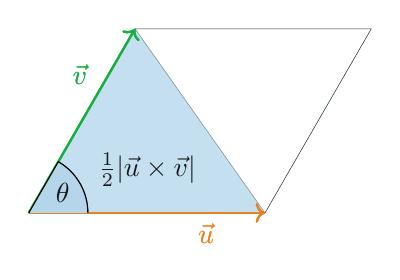
\begin{tikzpicture}
          \coordinate (A) at (0,0);
          \coordinate (B) at (0:3cm);
          \coordinate (D) at (60:2.7cm);
          \coordinate (C) at ($ (B) + (D) $);

          \tkzDrawPolygon[color=foreground](A,B,C,D);
          \draw[fill=title!50] (0,0) -- (60:.75cm) arc (60:0:.75cm);
          \draw[->,thick,hilight] (0,0) -- node[near end, below] {$\vec u$} (B);
          \draw[->,thick,vhilight] (0,0) -- node[near end, left=4pt] {$\vec v$} (D);
          \draw(30:0.5cm) node {\color{background}$\theta$};

          \visible<2->{
            %\draw[title,thick,->] (0,0) -- node[below] {$\vec{v}_{\vec{u}}$} (0:2.45134221cm);
            \tkzDrawPolygon[fill=title,opacity=0.4](A,B,D);
            \draw (20:1.6cm) node {\color{background}$\frac{1}{2}\lvert \vec{u} \times \vec{v} \rvert$};
            \draw[->,thick,hilight] (0,0) -- node[near end, below] {$\vec u$} (B);
            \draw[->,thick,vhilight] (0,0) -- node[near end, left=4pt] {$\vec v$} (D);
            \draw[fill=title!50] (0,0) -- (60:.75cm) arc (60:0:.75cm);
            \draw(30:0.5cm) node {\color{background}$\theta$};
          }
        \end{tikzpicture}
      \end{figure}
    \end{column}
    \begin{column}{0.6\textwidth}
      \begin{itemize}
        \item Allows us to calculate the area of the triangle formed by $\vec u$ and $\vec v$.
          \[
            \frac{\lvert \vec{u} \times \vec{v} \rvert}{2}
          \]
        \onslide<3->
        \item And can tell us if the angle between $\vec u$ and $\vec v$ is positive or negative.
          \begin{align*}
            \lvert \vec{u} \times \vec{v} \rvert &< 0 \quad\text{ iff }\quad \theta < \pi \\
            \lvert \vec{u} \times \vec{v} \rvert &= 0 \quad\text{ iff }\quad \theta = \pi \\
            \lvert \vec{u} \times \vec{v} \rvert &> 0 \quad\text{ iff }\quad \theta > \pi
          \end{align*}
      \end{itemize}
    \end{column}
  \end{columns}
\end{frame}

\begin{frame}[plain]
  \begin{columns}
    \begin{column}{0.4\textwidth}
      \begin{figure}
        \footnotesize
        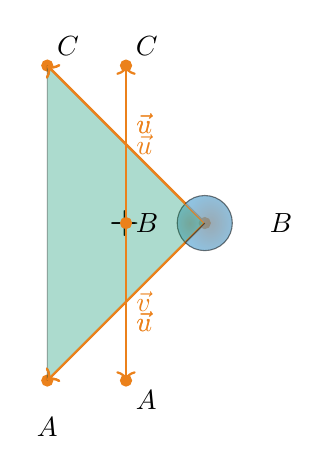
\begin{tikzpicture}
          \coordinate(A) at (0,0);
          \coordinate(B) at (2,2);
          \coordinate(C) at (0,4);
          \coordinate(D) at (-1,2);

          \coordinate(E) at (1,0);
          \coordinate(F) at (1,2);
          \coordinate(G) at (1,4);

          \visible<1-3>{
            \draw[hilight,fill] (A) circle[radius=2pt];
            \draw[hilight,fill] (B) circle[radius=2pt];
            \draw[hilight,fill] (C) circle[radius=2pt];
            \draw (A) node[below=10pt] {$A$};
            \draw (B) node[right=20pt] {$B$};
            \draw (C) node[above right] {$C$};
          }

          \visible<1-2>{
            \draw[thick,hilight,->] (B) -- node[above right] {$\vec v$} (C);
            \draw[thick,hilight,->] (B) -- node[below right] {$\vec u$} (A) ;
          }

          \visible<2>{
            \tkzDrawPolygon[fill=title,opacity=0.3](A,B,C);
            \draw (B) node[left=20pt] {\Large$+$};
            \draw[outer color=title,fill=title,opacity=0.5] (B) -- ++(135:.35cm) arc (135:225:.35cm);
          }

          \visible<3>{
            \tkzDrawPolygon[fill=vhilight,opacity=0.2](A,B,C);
            \draw (B) node[left=20pt] {\Large$-$};
            \draw[thick,hilight,->] (B) -- node[above right] {$\vec u$} (C);
            \draw[thick,hilight,->] (B) -- node[below right] {$\vec v$} (A) ;
            \draw[outer color=title,fill=title,opacity=0.5] (B) -- ++(225:.35cm) arc (225:495:.35cm);
          }

          \visible<4>{
            \draw[thick,hilight,->] (F) -- node[right] {$\vec v$} (E);
            \draw[thick,hilight,->] (F) -- node[right] {$\vec u$} (G) ;
            \draw[hilight,fill] (E) circle[radius=2pt];
            \draw[hilight,fill] (F) circle[radius=2pt];
            \draw[hilight,fill] (G) circle[radius=2pt];
            \draw (E) node[below right] {$A$};
            \draw (F) node[right] {$B$};
            \draw (G) node[above right] {$C$};
          }

        \end{tikzpicture}
      \end{figure}
    \end{column}
    \begin{column}{0.7\textwidth}
      %\footnotesize
      \begin{itemize}
        \only<1-2>{
          \item Given three points $A$, $B$ and $C$, we want to know if they form
            a counter-clockwise angle in that order.
            \[
              A \rightarrow B \rightarrow C
            \]
          }
        \only<2>{
          \item We can examine the cross product of and the area of the triangle formed by
            \begin{align*}
              \vec{u} = B - C &\quad \vec{v} = B - A \\
              \vec{u} &\times \vec{v} > 0
            \end{align*}
        }

        \only<3->{
          \item The points in the reverse order do not form a counter clockwise angle.
            \[
              C \rightarrow B \rightarrow A
            \]
          \item In the reverse order the vectors swap places
            \begin{align*}
              \vec{u} = B - A &\quad \vec{v} = B - C \\
              \vec{u} &\times \vec{v} < 0
            \end{align*}
        }

        \only<4>{
          \item If the points $A$, $B$ and $C$ are on the same line, then the area will be $0$.
        }
      \end{itemize}
    \end{column}
  \end{columns}
\end{frame}

\begin{frame}[plain,fragile]
  \vspace{20pt}
  \begin{minted}{cpp}
double cross(P(a), P(b)) {
    return real(a)*imag(b) - imag(a)*real(b);
}
double ccw(P(a), P(b), P(c)) {
    return cross(b - a, c - b);
}
bool collinear(P(a), P(b), P(c)) {
    return abs(ccw(a, b, c)) < EPS;
}
  \end{minted}
\end{frame}

\begin{frame}[plain]
  Very common task is to find the intersection of two lines or line segments.
  \begin{itemize}
    \onslide<2->
    \item Given a pair of points $(x_0, y_0)$, $(x_1, y_1)$, representing a
      line we want to start by obtaining the form $Ax + By = C$.
    \onslide<3->
    \item We can do so by setting
      \begin{align*}
        A &= y_1 - y_0 \\
        B &= x_0 - x_1 \\
        C &= A\cdot x_0 + B\cdot y_1
      \end{align*}
    \onslide<4->
    \vspace{-10pt}
    \item If we have two lines given by such equations, we simply need to solve
      for the two unknowns, $x$ and $y$.
  \end{itemize}
\end{frame}

\begin{frame}[plain]
  For two lines
  \begin{align*}
    A_0 x + B_0 y = C_0  \\
    A_1 x + B_1 y = C_1
  \end{align*}
  The intersection point is
  \begin{align*}
      x &= \frac{(B_1 \cdot C_0 - B_0 \cdot C_1)}{D} \\
      y &= \frac{(A_0 \cdot C_1 - A_1 \cdot C_0)}{D}
  \end{align*}
  Where
  \[
    D = A_0 \cdot B_1 - A_1 \cdot B_0
  \]
\end{frame}

%\begin{frame}[plain,fragile]
  %Quite similar problem is to find the intersections of two circles.
  %\begin{columns}
    %\begin{column}{0.6\textwidth}
      %\begin{figure}
        %\begin{tikzpicture}[auto,swap]
          %\scriptsize
          %\coordinate (A) at (0,0);
          %\coordinate (B) at (3,0);

          %\coordinate (P) at (1.2083333,0);
          %\coordinate (Q) at (1.2083333,0.88878037);
          %\coordinate (R) at (1.2083333,-0.88878037);

          %\draw[title,thick] (A) -- node[above left] {$r_A$} (Q);
          %\draw[title,thick] (B) -- node[above right] {$r_B$} (Q);

          %\draw (A) node[left] {\scriptsize$A$};
          %\draw (B) node[right] {\scriptsize$B$};
          %\draw[fill,vhilight] (A) circle[radius=1.2pt];
          %\draw[fill,vhilight] (B) circle[radius=1.2pt];
          %\draw[hilight,thick] (A) circle[radius=1.5cm];
          %\draw[hilight,thick] (B) circle[radius=2cm];

          %\visible<1-5>{
            %\draw[vhilight,thick] (A) --  node[below,xshift=5pt] {\scriptsize$d$} (B);
          %}

          %\visible<6->{
            %\draw[gray,thick] (A) circle[radius=1.5cm];
            %\draw[gray,thick] (B) circle[radius=2cm];
            %\draw[fill,vhilight] (A) circle[radius=1.2pt];
            %\draw[fill,vhilight] (B) circle[radius=1.2pt];

            %\draw[gray,thick] (P) -- (R);
            %\draw[hilight,thick] (Q) -- node[right=7pt] {$h$} (P);

            %\draw[vhilight, thick] (A) -- node[below] {$a$} (P);
            %\draw[vhilight, thick] (B) -- node[below] {$b$} (P);

            %\draw[fill,hilight] (P) circle[radius=1.2pt];
            %\draw[fill,hilight] (Q) circle[radius=1.2pt];
            %\draw[fill,hilight] (R) circle[radius=1.2pt];
          %}

        %\end{tikzpicture}
      %\end{figure}
    %\end{column}
    %\begin{column}{0.5\textwidth}
      %\footnotesize
      %\only<2-5>{
        %\begin{itemize}
            %\onslide<2-5>{
            %\item If $d > r_0 + r_1$ the circles do not intersect.
            %}
            %\onslide<3-5>{
            %\item If $d < \lvert r_0 - r_1 \rvert $, one circles is contained within the other.
            %}
            %\onslide<4-5>{
            %\item If $d = 0$ and $r_0 = r_1$, the circles are the same.
            %}
            %\onslide<5>{
            %\item Let's look at the last case.
            %}
        %\end{itemize}
      %}
      %\only<6->{
          %\begin{itemize}
            %\onslide<6->{
            %\item We can solve for the vectors $a$ and $h$ from the equations
                %\[
                %a^2 + h^2 = r_0^2 \quad b^2 + h^2 = r_1^2
                %\]
            %}
            %\onslide<7->{
            %\item We get
                %\[
                %a = \frac{r_A^2 - r_B^2 + d^2)}{2\cdot d}
                %\]
                %\[
                %h^2 = r_A^2 - a^2
                %\]
            %}
        %\end{itemize}
      %}
    %\end{column}
  %\end{columns}
%\end{frame}

%\begin{frame}[plain,fragile]
  %\footnotesize
  %\begin{minted}{cpp}
%#define C(p, r) const point &p, double r
%int intersect(C(A, rA), C(B, rB), point & res1, point & res2) { 
    %double d = abs(B - A);
    %if ( rA + rB <  d - EPS || d < abs(rA - rB) - EPS){
      %return 0;
    %}
    %double a = (rA*rA - rB*rB + d*d) / 2*d;
    %double h = sqrt(rA*rA - a*a);
    %point v = normalize(B - A, a);
    %u = normalize(rotate(B-A), h);
    %res1 = A + v + u;
    %res2 = A + v - u;
    %if (abs(u) < EPS){
        %return 1;
    %}
    %return 2;
%}
  %\end{minted}
%\end{frame}

\begin{frame}[plain]
  \begin{columns}
    \begin{column}{0.4\textwidth}
      \begin{figure}
        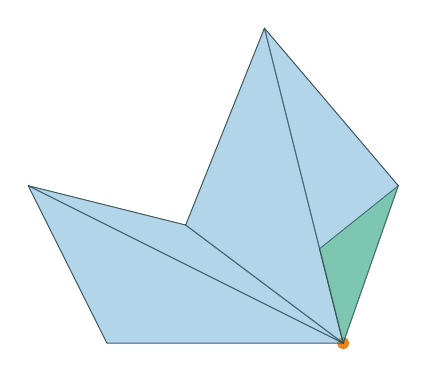
\begin{tikzpicture}
          \coordinate(A) at (0,0);
          \coordinate(B) at (3,0);
          \coordinate(C) at (2.7,1.2);
          \coordinate(D) at (3.7,2);
          \coordinate(E) at (2,4);
          \coordinate(F) at (1,1.5);
          \coordinate(G) at (-1,2);

          \tkzDrawPolygon[color=foreground](A,B,C,D,E,F,G);

          \visible<3->{
            \draw[fill,hilight] (B) circle[radius=2pt];
          }

          \visible<4>{
            \tkzDrawPolygon[color=foreground,fill=title,opacity=0.3,thin](A,B,G);
          }

          \visible<5>{
            \tkzDrawPolygon[color=foreground,fill=title,opacity=0.3,thin](B,G,F);
          }

          \visible<6>{
            \tkzDrawPolygon[color=foreground,fill=title,opacity=0.3,thin](B,F,E);
          }

          \visible<7>{
            \tkzDrawPolygon[color=foreground,fill=title,opacity=0.3,thin](B,E,D);
          }

          \visible<8>{
            \tkzDrawPolygon[color=foreground,fill=vhilight,opacity=0.2,thin](B,D,C);
          }

          \visible<9>{
            \tkzDrawPolygon[color=foreground,fill=title,opacity=0.3,thin](A,B,G);
            \tkzDrawPolygon[color=foreground,fill=title,opacity=0.3,thin](B,G,F);
            \tkzDrawPolygon[color=foreground,fill=title,opacity=0.3,thin](B,F,E);
            \tkzDrawPolygon[color=foreground,fill=title,opacity=0.3,thin](B,E,D);
            \tkzDrawPolygon[color=foreground,fill=vhilight,opacity=0.2,thin](B,D,C);
          }
        \end{tikzpicture}
      \end{figure}
    \end{column}
    \begin{column}{0.6\textwidth}
      \begin{itemize}
        \item Polygons are represented by a list of points in the order
          representing the edges.
        \onslide<2->
        \item To calculate the area
          \begin{itemize}
            \onslide<3->
            \item We pick one starting point.
            \onslide<4->
            \item Go through all the other adjacent pair of points and sum the
              area of the triangulation.
            \onslide<8->
            \item Even if we sum up area outside the polygon, due to the cross
              product, it is subtracted later.
          \end{itemize}
      \end{itemize}
    \end{column}
  \end{columns}
\end{frame}

%\begin{frame}[plain,fragile]
  %\vspace{20pt}
  %%Very simple code.
  %\footnotesize
  %\begin{minted}{cpp}
%double polygon_area_signed(const vector<point> &p) {
    %double area = 0;
    %int cnt = size(p);
    %for (int i = 1; i + 1 < cnt; i++){
        %area += cross(p[i] - p[0], p[i + 1] - p[0])/2;
    %}
    %return area;
%}
%double polygon_area(vector<point> &p) {
    %return abs(polygon_area_signed(p));
%}
  %\end{minted}
%\end{frame}

\begin{frame}[plain,fragile]
  \begin{itemize}
    \item Given a set of points, we want to find the convex hull of the points.
    \onslide<2->
    \item The convex hull of points can be visualized as the shape formed by a rubber band around the set of points.
  \end{itemize}
  \onslide<3->
  \begin{figure}
    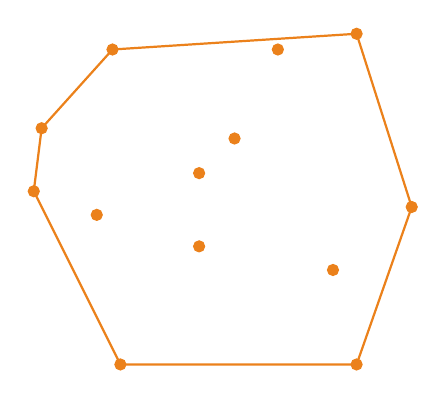
\begin{tikzpicture}
      \coordinate(A) at (0,0);
      \coordinate(B) at (3,0);
      \coordinate(C) at (2.7,1.2);
      \coordinate(D) at (3.7,2);
      \coordinate(E) at (2,4);
      \coordinate(F) at (1,1.5);
      \coordinate(G) at (-1,3);
      \coordinate(H) at (3,4.2);
      \coordinate(I) at (1,2.43);
      \coordinate(J) at (1.45, 2.87);
      \coordinate(K) at (-0.1, 4);
      \coordinate(L) at (-1.1,2.2);
      \coordinate(M) at (-0.3,1.9);

      \draw[fill,hilight] (A) circle[radius=2pt];
      \draw[fill,hilight] (B) circle[radius=2pt];
      \draw[fill,hilight] (C) circle[radius=2pt];
      \draw[fill,hilight] (D) circle[radius=2pt];
      \draw[fill,hilight] (E) circle[radius=2pt];
      \draw[fill,hilight] (F) circle[radius=2pt];
      \draw[fill,hilight] (G) circle[radius=2pt];
      \draw[fill,hilight] (H) circle[radius=2pt];
      \draw[fill,hilight] (I) circle[radius=2pt];
      \draw[fill,hilight] (J) circle[radius=2pt];
      \draw[fill,hilight] (K) circle[radius=2pt];
      \draw[fill,hilight] (L) circle[radius=2pt];
      \draw[fill,hilight] (M) circle[radius=2pt];

      \visible<4->{
        \draw[hilight,thick] (A) -- (B) -- (D) -- (H) -- (K) -- (G) -- (L) -- cycle;
      }
    \end{tikzpicture}
  \end{figure}
\end{frame}

\begin{frame}[plain,fragile]
  \vspace{20pt}
  Graham scan:
  \begin{itemize}
    \onslide<2->
    \item Pick the point $p_0$ with the lowest $y$ coordinate.
    \onslide<3->
    \item Sort all the points by polar angle with $p_0$.
    \onslide<4->
    \item Iterate through all the points
    \onslide<5->
    \item If the current point forms a clockwise angle with the last two
      points, remove last point from the convex set.
    \onslide<6->
    \item Otherwise, add the current point to the convex set.
  \end{itemize}
  \onslide<7->
  Time complexity $O(N \log N)$.
\end{frame}

\begin{frame}[plain]
  \begin{figure}
    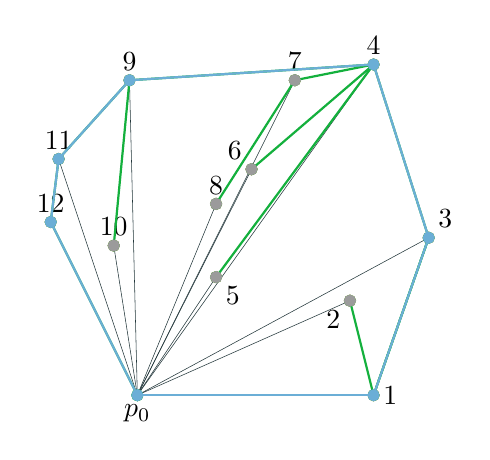
\begin{tikzpicture}
      \coordinate(A) at (0,0);
      \coordinate(B) at (3,0);
      \coordinate(C) at (2.7,1.2);
      \coordinate(D) at (3.7,2);
      \coordinate(E) at (2,4);
      \coordinate(F) at (1,1.5);
      \coordinate(G) at (-1,3);
      \coordinate(H) at (3,4.2);
      \coordinate(I) at (1,2.43);
      \coordinate(J) at (1.45, 2.87);
      \coordinate(K) at (-0.1, 4);
      \coordinate(L) at (-1.1,2.2);
      \coordinate(M) at (-0.3,1.9);

      %\draw[fill,hilight] (A) circle[radius=2pt];
      \onslide<2->{
        \draw[fill,hilight] (B) circle[radius=2pt];
        \draw[fill,hilight] (C) circle[radius=2pt];
        \draw[fill,hilight] (D) circle[radius=2pt];
        \draw[fill,hilight] (E) circle[radius=2pt];
        \draw[fill,hilight] (F) circle[radius=2pt];
        \draw[fill,hilight] (G) circle[radius=2pt];
        \draw[fill,hilight] (H) circle[radius=2pt];
        \draw[fill,hilight] (I) circle[radius=2pt];
        \draw[fill,hilight] (J) circle[radius=2pt];
        \draw[fill,hilight] (K) circle[radius=2pt];
        \draw[fill,hilight] (L) circle[radius=2pt];
        \draw[fill,hilight] (M) circle[radius=2pt];
        \draw[fill,vhilight] (A) circle[radius=2pt];
      }

      \visible<3-4>{
        \draw[very thin,foreground] (A) -- (B);
        \draw[very thin,foreground] (A) -- (C);
        \draw[very thin,foreground] (A) -- (D);
        \draw[very thin,foreground] (A) -- (E);
        \draw[very thin,foreground] (A) -- (F);
        \draw[very thin,foreground] (A) -- (G);
        \draw[very thin,foreground] (A) -- (H);
        \draw[very thin,foreground] (A) -- (I);
        \draw[very thin,foreground] (A) -- (J);
        \draw[very thin,foreground] (A) -- (K);
        \draw[very thin,foreground] (A) -- (L);
        \draw[very thin,foreground] (A) -- (M);
      }

      \visible<4->{
        \draw (A) node[below] {$p_0$};
        \draw (B) node[right] {$1$};
        \draw (C) node[below left] {$2$};
        \draw (D) node[above right] {$3$};
        \draw (E) node[above] {$7$};
        \draw (F) node[below right] {$5$};
        \draw (G) node[above] {$11$};
        \draw (H) node[above] {$4$};
        \draw (I) node[above] {$8$};
        \draw (J) node[above left] {$6$};
        \draw (K) node[above] {$9$};
        \draw (L) node[above] {$12$};
        \draw (M) node[above] {$10$};
      }

      \visible<5->{
        \draw[fill,vhilight] (B) circle[radius=2pt];

      }
      \visible<5-7>{
        \draw[fill,vhilight] (C) circle[radius=2pt];
      }
      \visible<5>{
        \draw[thick, vhilight] (B) -- (C);
      }
      \visible<5->{
        \draw[thick, vhilight] (A) -- (B);
      }
      \visible<6->{
        \draw[fill,gray] (C) circle[radius=2pt];
      }
      \visible<6->{
        \draw[fill,vhilight] (D) circle[radius=2pt];
      }
      \visible<6->{
        \draw[thick, vhilight] (B) -- (D);
      }
      %\visible<7->{
        %\draw[fill,title] (A) circle[radius=2pt];
        %\draw[thick, title] (A) -- (B);
      %}
      \visible<7>{
        \draw[thick, vhilight] (B) -- (D);
      }
      %\visible<8->{
        %\draw[fill,title] (B) circle[radius=2pt];
        %\draw[thick, title] (B) -- (D);
      %}
      \visible<7->{
        \draw[thick, vhilight] (D) -- (H);
      }
      \visible<7->{
        \draw[fill,vhilight] (H) circle[radius=2pt];
      }
      \visible<8>{
        \draw[thick, vhilight] (H) -- (F);
        \draw[fill,vhilight] (F) circle[radius=2pt];
      }
      \visible<9->{
        \draw[fill,gray] (F) circle[radius=2pt];
      }
      \visible<9>{
        \draw[thick, vhilight] (H) -- (J);
        \draw[fill,vhilight] (J) circle[radius=2pt];
      }
      \visible<10->{
        \draw[fill,gray] (J) circle[radius=2pt];
      }
      \visible<10-11>{
        \draw[thick, vhilight] (H) -- (E);
        \draw[fill,vhilight] (E) circle[radius=2pt];
      }
      %\visible<11-12>{
        %\draw[fill,gray] (E) circle[radius=2pt];
      %}
      \visible<11>{
        \draw[thick, vhilight] (E) -- (I);
        \draw[fill,vhilight] (I) circle[radius=2pt];
      }

      \visible<12->{
        \draw[fill,gray] (E) circle[radius=2pt];
        \draw[fill,gray] (I) circle[radius=2pt];
      }
      \visible<12->{
        \draw[thick, vhilight] (H) -- (K);
      }
      \visible<12->{
        \draw[fill,vhilight] (K) circle[radius=2pt];
      }
      %\visible<13->{
        %\draw[thick, title] (D) -- (H);
        %\draw[fill,title] (D) circle[radius=2pt];
      %}
      \visible<13>{
        \draw[thick, vhilight] (K) -- (M);
        \draw[fill,vhilight] (M) circle[radius=2pt];
      }
      \visible<14->{
        \draw[fill,gray] (M) circle[radius=2pt];
      }
      \visible<14->{
        \draw[thick, vhilight] (K) -- (G);
      }
      \visible<14->{
        \draw[fill,vhilight] (G) circle[radius=2pt];
      }
      %\visible<15->{
        %\draw[fill,title] (H) circle[radius=2pt];
        %\draw[thick, title] (H) -- (K);
      %}
      \visible<15->{
        \draw[thick, vhilight] (G) -- (L);
        \draw[fill,vhilight] (L) circle[radius=2pt];
      }
      %\visible<16->{
        %\draw[fill,title] (K) circle[radius=2pt];
        %\draw[thick, title] (K) -- (G);
      %}
      \visible<16>{
        \draw[thick, vhilight] (L) -- (A);
        \draw[fill,vhilight] (A) circle[radius=2pt];
      }
      \visible<17->{
        \draw[thick, title] (A) -- (B);
        \draw[thick, title] (B) -- (D);
        \draw[thick, title] (D) -- (H);
        \draw[thick, title] (H) -- (K);
        \draw[thick, title] (K) -- (G);
        \draw[thick, title] (G) -- (L);
        \draw[thick, title] (L) -- (A);
        \draw[fill,title] (A) circle[radius=2pt];
        \draw[fill,title] (B) circle[radius=2pt];
        \draw[fill,title] (D) circle[radius=2pt];
        \draw[fill,title] (H) circle[radius=2pt];
        \draw[fill,title] (K) circle[radius=2pt];
        \draw[fill,title] (G) circle[radius=2pt];
        \draw[fill,title] (L) circle[radius=2pt];
      }

    \end{tikzpicture}
  \end{figure}
\end{frame}

\begin{frame}[plain,fragile]
  \footnotesize
  \begin{minted}{cpp}
point hull[MAXN];
bool cmp(const point &a, const point &b) {
  return abs(real(a) - real(b)) > EPS ?
    real(a) < real(b) : imag(a) < imag(b); }
int convex_hull(vector<point> p) {
    int n = size(p), l = 0;
    sort(p.begin(), p.end(), cmp);
    for (int i = 0; i < n; i++) {
        if (i > 0 && p[i] == p[i - 1]) 
            continue;
        while (l >= 2 && ccw(hull[l - 2], hull[l - 1], p[i]) >= 0)
            l--;
        hull[l++] = p[i]; }
    int r = l;
    for (int i = n - 2; i >= 0; i--) {
        if (p[i] == p[i + 1])
            continue;
        while (r - l >= 1 && ccw(hull[r - 2], hull[r - 1], p[i]) >= 0)
            r--;
        hull[r++] = p[i]; }
    return l == 1 ? 1 : r - 1; }
  \end{minted}
\end{frame}

\begin{frame}[plain]
  \vspace{40pt}
  Many other algorithms exist
  \begin{itemize}
    \onslide<2->
    \item Gift wrapping aka Jarvis march.
    \onslide<3->
    \item Quick hull, similar idea to quicksort.
    \onslide<4->
    \item Divide and conquer.
  \end{itemize}
  \onslide<5->
  Some can be extended to three dimensions, or higher.
\end{frame}

\begin{frame}[plain]
  Simple algorithm to check if a point is in a convex polygon.
  \begin{columns}
    \begin{column}{0.6\textwidth}
      \begin{figure}
        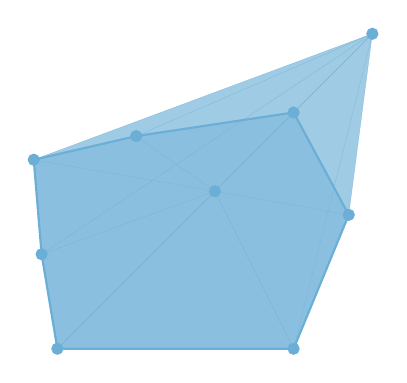
\begin{tikzpicture}
          \coordinate(A) at (0,0);
          \coordinate(B) at (3,0);
          \coordinate(C) at (3.7,1.7);
          \coordinate(D) at (3,3);
          \coordinate(E) at (1, 2.7);
          \coordinate(F) at (-0.3,2.4);
          \coordinate(G) at (-0.2,1.2);

          \coordinate(P) at (4,4);
          \coordinate(Q) at (2,2);

          \draw[fill,title] (A) circle[radius=2pt];
          \draw[fill,title] (B) circle[radius=2pt];
          \draw[fill,title] (C) circle[radius=2pt];
          \draw[fill,title] (D) circle[radius=2pt];
          \draw[fill,title] (E) circle[radius=2pt];
          \draw[fill,title] (F) circle[radius=2pt];
          \draw[fill,title] (G) circle[radius=2pt];

          \visible<1-10>{
            \draw[fill,title] (P) circle[radius=2pt];
          }

          \visible<11->{
            \draw[fill,title] (Q) circle[radius=2pt];
          }

          \draw[title,thick] (A) -- (B) -- (C) -- (D) -- (E) -- (F) -- (G) -- cycle;
          \visible<2>{
            \tkzDrawPolygon[color=title,fill=title,opacity=0.4,ultra thin](A,B,C,D,E,F,G);
          }
          \visible<3-10>{
            \tkzDrawPolygon[color=title,fill=title,opacity=0.4,ultra thin](A,B,P);
          }
          \visible<4-10>{
            \tkzDrawPolygon[color=title,fill=title,opacity=0.4,ultra thin](B,C,P);
          }
          \visible<5-10>{
            \tkzDrawPolygon[color=title,fill=title,opacity=0.4,ultra thin](C,D,P);
          }
          \visible<6-10>{
            \tkzDrawPolygon[color=title,fill=title,opacity=0.4,ultra thin](D,E,P);
          }
          \visible<7-10>{
            \tkzDrawPolygon[color=title,fill=title,opacity=0.4,ultra thin](E,F,P);
          }
          \visible<8-10>{
            \tkzDrawPolygon[color=title,fill=title,opacity=0.4,ultra thin](F,G,P);
          }
          \visible<9-10>{
            \tkzDrawPolygon[color=title,fill=title,opacity=0.4,ultra thin](G,A,P);
          }

          \visible<11->{
            \tkzDrawPolygon[color=title,fill=title,opacity=0.4,ultra thin](A,B,Q);
          }
          \visible<12->{
            \tkzDrawPolygon[color=title,fill=title,opacity=0.4,ultra thin](B,C,Q);
          }
          \visible<13->{
            \tkzDrawPolygon[color=title,fill=title,opacity=0.4,ultra thin](C,D,Q);
          }
          \visible<14->{
            \tkzDrawPolygon[color=title,fill=title,opacity=0.4,ultra thin](D,E,Q);
          }
          \visible<15->{
            \tkzDrawPolygon[color=title,fill=title,opacity=0.4,ultra thin](E,F,Q);
          }
          \visible<16->{
            \tkzDrawPolygon[color=title,fill=title,opacity=0.4,ultra thin](F,G,Q);
          }
          \visible<17->{
            \tkzDrawPolygon[color=title,fill=title,opacity=0.4,ultra thin](G,A,Q);
          }

        \end{tikzpicture}
      \end{figure}
    \end{column}
    \begin{column}{0.5\textwidth}
      \footnotesize
      \begin{itemize}
        \onslide<2->
        \item We start by calculating the area of the polygon.
        \onslide<3->
        \item To check if our point is contained in the polygon we sum up the
          area of the triangles formed the point and every two adjacent points.
        \onslide<10->
        \item The total area of the triangles is equal to the area of the
          polygon iff the point is inside the polygon.
      \end{itemize}
    \end{column}
  \end{columns}
\end{frame}

\begin{frame}[plain]
  \vspace{40pt}
  How about non convex polygon?
  \begin{itemize}
    \onslide<2->
    \item The \emph{even-odd rule} algorithm.
    \onslide<3->
    \item We examine a ray passing through the polygon to the point.
    \onslide<4->
    \item If the ray crosses the boundary of the polygon, then it alternately
      goes from outside to inside, and outside to inside.
  \end{itemize}
\end{frame}

\begin{frame}[plain]
  \begin{columns}
    \begin{column}{0.6\textwidth}
      \begin{figure}
        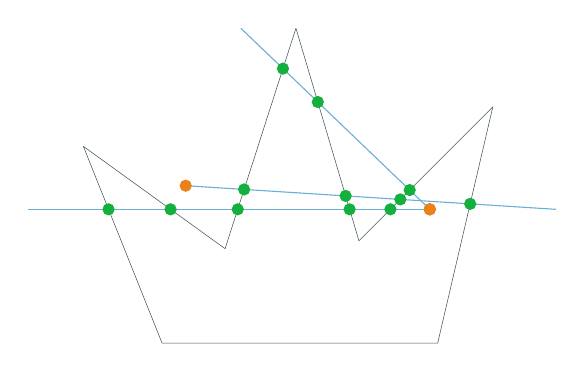
\begin{tikzpicture}
            \coordinate(A) at (0,0);
            \coordinate(B) at (3.5,0);
            \coordinate(C) at (2.7,1.2);
            \coordinate(D) at (4.2,3);
            \coordinate(E) at (2.5,1.3);
            \coordinate(F) at (1.7,4);
            \coordinate(G) at (0.8,1.2);
            \coordinate(H) at (-1,2.5);

            \coordinate(P) at (-1.7,1.7);
            \coordinate(Q) at (5,1.7);

            \coordinate(R) at (1,4);
            \coordinate(S) at (0.3, 2);

            \coordinate(O) at (3.4, 1.7);
            \onslide<1-2>{
              \draw[fill,hilight] (O) circle[radius=2pt];
            }

            \tkzInterLL(B,D)(P,Q) \tkzGetPoint{LL1};
            \tkzInterLL(D,E)(P,Q) \tkzGetPoint{LL2};
            \tkzInterLL(E,F)(P,Q) \tkzGetPoint{LL3};
            \tkzInterLL(F,G)(P,Q) \tkzGetPoint{LL4};
            \tkzInterLL(G,H)(P,Q) \tkzGetPoint{LL5};
            \tkzInterLL(H,A)(P,Q) \tkzGetPoint{LL6};

            \tkzInterLL(D,E)(R,O) \tkzGetPoint{LL7};
            \tkzInterLL(E,F)(R,O) \tkzGetPoint{LL8};
            \tkzInterLL(F,G)(R,O) \tkzGetPoint{LL9};

            \tkzInterLL(B,D)(S,Q) \tkzGetPoint{LL10};
            \tkzInterLL(D,E)(S,Q) \tkzGetPoint{LL11};
            \tkzInterLL(E,F)(S,Q) \tkzGetPoint{LL12};
            \tkzInterLL(F,G)(S,Q) \tkzGetPoint{LL13};

            \tkzDrawPolygon[color=foreground,opacity=0.85](A,B,D,E,F,G,H);

            \onslide<2-4>{
              %\tkzDrawPolygon[color=foreground,opacity=0.7](A,B,D,E,F,G,H);
              \draw[vhilight,title] (P) -- (O);
              \draw[fill,hilight] (O) circle[radius=2pt];
            }

            \onslide<3-4>{
              \draw[fill,vhilight] (LL2) circle[radius=2pt];
              \draw[fill,vhilight] (LL3) circle[radius=2pt];
              \draw[fill,vhilight] (LL4) circle[radius=2pt];
              \draw[fill,vhilight] (LL5) circle[radius=2pt];
              \draw[fill,vhilight] (LL6) circle[radius=2pt];
            }

            \onslide<5-6>{
              \draw[vhilight,title] (R) -- (O);
              \draw[fill,hilight] (O) circle[radius=2pt];
            }

            \onslide<6>{
              \draw[fill,vhilight] (LL7) circle[radius=2pt];
              \draw[fill,vhilight] (LL8) circle[radius=2pt];
              \draw[fill,vhilight] (LL9) circle[radius=2pt];
            }

            \onslide<7-8>{
              %\tkzDrawPolygon[color=foreground,opacity=0.7](A,B,D,E,F,G,H);
              \draw[vhilight,title] (Q) -- (S);
              \draw[fill,hilight] (S) circle[radius=2pt];
            }

            \onslide<8>{
              \draw[fill,vhilight] (LL10) circle[radius=2pt];
              \draw[fill,vhilight] (LL11) circle[radius=2pt];
              \draw[fill,vhilight] (LL12) circle[radius=2pt];
              \draw[fill,vhilight] (LL13) circle[radius=2pt];
            }

        \end{tikzpicture}
      \end{figure}
    \end{column}
    \begin{column}{0.5\textwidth}
      \begin{itemize}
        \onslide<2->
        \item Ray from the outside of the polygon to the point.
        \onslide<3->
        \item Count the number of intersection points.
        \onslide<4->
        \item If odd, then the point is inside the polygon.
        \item If even, then the point is outside the polygon.
        \onslide<5->
        \item Does not matter which ray we pick.
      \end{itemize}
    \end{column}
  \end{columns}
\end{frame}

\begin{frame}[plain]{An algorithm}
	\begin{itemize}
        \item Computational geometry has a lot of impressive and technical algorithms.
        \item The most famous one is probably Delaunay triangulation.
        \item But that one is a bit too hard for this course, so we will instead look at the classical closest point algorithm.
        \item We are given $n$ points in the plan, find the pair of points that are closest to one another.
        \item We can clearly solve this in $\mathcal{O}(n^2)$ time, but can we do better?
    \end{itemize}
\end{frame}

\begin{frame}[plain]{Divide and conquer}
	\begin{itemize}
        \item We sort the points by $x$-coordinate and split the list in half.
        \item Let $x_0$ be such that it's between the coordinates of the left and right halves.
        \item Start by solving each half recursively.
        \item We now have to find if there's some pair with one point in each half that does better.
        \item We can't simply try all pairs, that's too slow. Suppose the smallest distance we found recursively was $d$.
        \item Then we can ignore all points with $x$-coordinte outside $[x_0 - d, x_0 + d]$.
        \item Sort the points inside of this interval by their $y$-coordinate.
        \item The big trick is now that we only need to consider a few neighbours for each point.
    \end{itemize}
\end{frame}

\begin{frame}[plain]{Neighbours}
	\begin{itemize}
        \item Divide the area above $x_i$ into 8 squares, each with side length $d/2$.
        \item If he distance between all points in each half is at least $d$, then we can have at most each point per square.
        \item All points outside these squares are at a distance of at least $d$ from $x_i$, so we can ignore them.
        \item Thus we only need to look at the distance from $x_i$ to $x_j$ when $j - i \leq 7$.
    \end{itemize}
\end{frame}

\begin{frame}[plain]{Diagram}
	\begin{center}
		\begin{tikzpicture}
			\draw (-2, 0) -- (-2, 8);
			\draw (-2, 8) -- (2, 8);
			\draw (2, 8) -- (2, 0);
			\draw (2, 0) -- (-2, 0);
			\draw (0, 0) -- (0, 8);
			\draw (-2, 3) -- (2, 3);
			\draw (-2, 4) -- (2, 4);
			\draw (-2, 5) -- (2, 5);
			\draw (-1, 3) -- (-1, 5);
			\draw (1, 3) -- (1, 5);
			\node[draw, fill, circle, white] at (-3, 0) {}; %alignment
			\node[draw, fill, circle, white] at (3, 0) {}; %alignment

			\node[draw, fill, circle, inner sep = 0.5pt] at (1, 0.3) {};
			\node[draw, fill, circle, inner sep = 0.5pt] at (-1.9, 0.4) {};
			\node[draw, fill, circle, inner sep = 0.5pt] at (-0.3, 1.3) {};
			\node[draw, fill, circle, inner sep = 0.5pt] at (1.3, 3) {};
			\node[draw, fill, circle, inner sep = 0.5pt] at (0.5, 4.7) {};
			\node[draw, fill, circle, inner sep = 0.5pt] at (-0.6, 4.4) {};
			\node[draw, fill, circle, inner sep = 0.5pt] at (-1.9, 3.1) {};
			\node[draw, fill, circle, inner sep = 0.5pt] at (-0.3, 6.2) {};
			\node[draw, fill, circle, inner sep = 0.5pt] at (0.6, 7.5) {};
			\node at (1.4,3.1) {\tiny $i$};
        \end{tikzpicture}
    \end{center}
\end{frame}

\begin{frame}[plain]{Diagram}
	\begin{center}
		\begin{tikzpicture}
			\draw (-2, 0) -- (-2, 8);
			\draw (-2, 8) -- (2, 8);
			\draw (2, 8) -- (2, 0);
			\draw (2, 0) -- (-2, 0);
			\draw (0, 0) -- (0, 8);
			\draw (-2, 3) -- (2, 3);
			\draw (-2, 4) -- (2, 4);
			\draw (-2, 5) -- (2, 5);
			\draw (-1, 3) -- (-1, 5);
			\draw (1, 3) -- (1, 5);
			\node[draw, fill, circle, white] at (-3, 0) {}; %alignment
			\node[draw, fill, circle, white] at (3, 0) {}; %alignment

			\node[draw, fill, circle, inner sep = 0.5pt] at (1, 0.3) {};
			\node[draw, fill, circle, inner sep = 0.5pt] at (-1.9, 0.4) {};
			\node[draw, fill, circle, inner sep = 0.5pt] at (-0.3, 1.3) {};
			\node[draw, fill, circle, inner sep = 0.5pt] at (2, 3) {};
			\node[draw, fill, circle, inner sep = 0.5pt] at (0.05, 3) {};
			\node[draw, fill, circle, inner sep = 0.5pt] at (-0.05, 3) {};
			\node[draw, fill, circle, inner sep = 0.5pt] at (-2, 3) {};
			\node[draw, fill, circle, inner sep = 0.5pt] at (2, 5) {};
			\node[draw, fill, circle, inner sep = 0.5pt] at (0.05, 5) {};
			\node[draw, fill, circle, inner sep = 0.5pt] at (-0.05, 5) {};
			\node[draw, fill, circle, inner sep = 0.5pt] at (-2, 5) {};
			\node[draw, fill, circle, inner sep = 0.5pt] at (-0.3, 6.2) {};
			\node[draw, fill, circle, inner sep = 0.5pt] at (0.6, 7.5) {};
			\node at (1.9, 3.1) {\tiny $i$};
			\node at (-0.2, 6.3) {\tiny $j$};
        \end{tikzpicture}
    \end{center}
\end{frame}

\begin{frame}[plain]{Complexity}
	\begin{itemize}
        \item Each recursive call is $\mathcal{O}(n\log(n))$. 
        \item Thus by the master theorem the total complexity is $\mathcal{O}(n\log^2(n))$.
        \item If we sort the $y$ values as we go using mergesort, we can actually do each call in $\mathcal{O}(n)$.
        \item This way the complexity is actually $\mathcal{O}(n\log(n))$.
    \end{itemize}
\end{frame}

\end{document}

